%%%%%%%%%%%%%%%%%%%%%%%%%%%%%%%%%%%%%%%%%%%%%%%%%%%%%%%%%%%%%%%%%%%%%%%%%%%%%%%%
%2345678901234567890123456789012345678901234567890123456789012345678901234567890
%        1         2         3         4         5         6         7         8

\documentclass[letterpaper, 10 pt, conference]{ieeeconf}  % Comment this line out if you need a4paper

%\documentclass[a4paper, 10pt, conference]{ieeeconf}      % Use this line for a4 paper

\IEEEoverridecommandlockouts                              % This command is only needed if 
                                                          % you want to use the \thanks command

\overrideIEEEmargins                                      % Needed to meet printer requirements.

%In case you encounter the following error:
%Error 1010 The PDF file may be corrupt (unable to open PDF file) OR
%Error 1000 An error occurred while parsing a contents stream. Unable to analyze the PDF file.
%This is a known problem with pdfLaTeX conversion filter. The file cannot be opened with acrobat reader
%Please use one of the alternatives below to circumvent this error by uncommenting one or the other
%\pdfobjcompresslevel=0
%\pdfminorversion=4

% See the \addtolength command later in the file to balance the column lengths
% on the last page of the document

% The following packages can be found on http:\\www.ctan.org
\usepackage{graphics} % for pdf, bitmapped graphics files
\usepackage{epsfig} % for postscript graphics files
%\usepackage{mathptmx} % assumes new font selection scheme installed
%\usepackage{times} % assumes new font selection scheme installed
%\usepackage{amsmath} % assumes amsmath package installed
%\usepackage{amssymb}  % assumes amsmath package installed

\title{\LARGE \bf
A Hybrid Control Framework for Navigating Pedestrian Interaction at Mid-Block Intersections}


\author{Nitin R. Kapania$^{1}$, Sarah M Thornton, Francesco Borrelli, J Christian Gerdes% <-this % stops a space
\thanks{*This work was supported by the Hyundai Center of Excellence}% <-this % stops a space
\thanks{$^{1}$Nitin Kapania is with the Dept. of Mechanical Engineering, Stanford University, and is a visiting scholar at UC Berkeley}%
}


\begin{document}



\maketitle
\thispagestyle{empty}
\pagestyle{empty}


%%%%%%%%%%%%%%%%%%%%%%%%%%%%%%%%%%%%%%%%%%%%%%%%%%%%%%%%%%%%%%%%%%%%%%%%%%%%%%%%
\begin{abstract}

As autonomous vehicles (AVs) inch closer to reality, a central requirement for acceptance will be earning the trust of humans in everyday driving situations. In particular, the interaction between AVs and pedestrians is of
high importance, as every human is a pedestrian at some point of the day. This paper considers the interaction of a pedestrian and an autonomous vehicle at a mid-block, unsignalized intersection where there is ambiguity
over when the pedestrian should cross and when and how the vehicle should yield. By modeling pedestrian behavior through the concept of gap acceptance, the authors show that a hybrid controller with just four states allows an autonomous vehicle to successfully interact with a pedestrian across a continuous spectrum of possible crosswalk-entry behaviors. The controller is validated in simulation through comparison with a previously published control policy obtained through solution of a POMDP, and experimental results are provided on a Hyundai Genesis vehicle for a virtual pedestrian.  

\end{abstract}


%%%%%%%%%%%%%%%%%%%%%%%%%%%%%%%%%%%%%%%%%%%%%%%%%%%%%%%%%%%%%%%%%%%%%%%%%%%%%%%%
\section{Introduction}

\subsection{Motivation}

While autonomous vehicles have the potential to save thousands of lives every year and create tremendous societal benefits \cite{Fagnant2015}, widespread adoption is unlikely until AVs gain the broad trust of society. Given that every human is a pedestrian at some point during the day, one of the central ways that autonomous vehicles will be evaluated is through their interactions with pedestrians. In fact, recent events with industry leader Waymo highlight that AV-pedestrian interaction has still not been perfected\cite{MattRichtelandConorDougherty2015}. In general, interactions with pedestrians are complex, even for experienced human drivers. Issues such as lack of visibility, improper communication, poorly marked roads, and distraction on both the driver or pedestrian side can lead to accidents and fatalities. From 2015-2016, pedestrian fatalaties increased by 9\% to 5987, representing the highest number since 1990, and also representing 16\% of all automotive fatalities \cite{HighwayTrafficSafetyAdministration2016}. As autonomous vehicles inch closer to widespread adoption, they must have a clear control strategy for pedestrian interaction that can handle a wide variety of pedestrian behaviors while maintaining a reasonable flow of traffic.    

\subsection{Prior Art}

The need to further understand pedestrian behavior for autonomous driving has created growing body of interdisciplinary research. One branch of research has focused around modeling pedestrian behavior given various sensor inputs. Keller et al \cite{Keller2014} presented a study on pedestrian path prediction and action classification (e.g. crossing vs. waiting) using Gaussian process dynamical models and trajectory matching from optical data. Several other techniques for pedestrian trajectory prediction have been proposed, including LQR \cite{Batkovic}, set-based reachability analysis \cite{Koschi2018}, and Markov processes \cite{Karasev2016} 

Another branch of literature is focused on developing binary predictive models for pedestrian crossing. While typically studied for purposes of road design, this body of literature holds promising insights for AV designers. For example, Schroeder and Rouphail \cite{Schroeder2011} explored factors associated with driver yielding behavior at unsignalized pedestrian crossings. Using logistic regression, the authors found that drivers are more likely to yield to assertive pedestrians who walk briskly in their approach to a crosswalk. Kadali and Perumal \cite{RaghuramKadali2012} studied the ``gap acceptance" behavior of pedestrians at mid-block crosswalks through a video graphic survey, and found that the gap accepted for crossing was explained by factors such as crossing direction, vehicle speed, and pedestrian age. Yannis et al. \cite{Yannis2013} and \cite{Sun2002} also found that gap acceptance was influenced by the size of the oncoming vehicle and the presence of other pedestrians.  Lee and Aty \cite{Lee2005} studied interactions in the form of crashes, and found crashes were linked with higher daily traffic. 

Finally, a small but rapidly growing body of literature specifically studies the interaction between pedestrians and autonomous vehicles at crosswalks. An excellent review of these studies was conducted by \cite{Rasouli}. As an example, Rothenbucher et al. \cite{Rothenbucher2016} studied the interaction between pedestrians and driverless vehicles by constructing a car seat costume to disguise a driver. The authors noted that pedestrians overall managed interactions at crosswalks effectively, but later mentioned increased uncertainty about the autonomous vehicles behavior. To improve the issue of trust, several researchers have developed external interfaces to more clearly broadcast the intent of the autonomous vehicle \cite{Matthews}, \cite{Lagstrom2015}. 

Several real-world studies of AV-pedestrian interaction note that once a local population learned a vehicle was programmed to be perfectly safe, pedestrians would regularly take advantage of the AV and walk in front of it. \cite{Madigan}. This illustrates an issue with automated driving in that an overly conservative crossing algorithm will often be taken advantage of or cause confusion among pedestrians. Camara et al \cite{Camara2018} attempted to model the natural negotation for priority between a pedestrian and an AV at an intersection using the framework of ``sequential chicken" adopted from game theory. Chen et al. \cite{Chen} notes the need for a tradeoff between passive and aggressive driving behavior, and developed a stochastic model of pedestrian behavior to evaluate proposed AV control policies. Control polices for pedestrian interaction are also developed by \cite{Bandyopadhyay}, who proposes a Mixed-observable Markov Decision Process (MOMDP) to incorporate the intention uncertainty of a pedestrian. A POMDP formulation is also proposed by Thornton \cite{Thornton2018}, who proposes navigation of the pedestrian uncertainty through value-sensitive design. 

\subsection{Statement of Contributions}
While there exists a wide body of research on the distinct subjects of pedestrian modeling and AV control, there is a lack of research that combines the two. In other words, significant research has been conducted to understand the likelihood of pedestrian crossing given certain traffic conditions and pedestrian demographics \cite{Schroeder2011} -\cite{Lee2005}, and a small but growing body of literature develops control strategies for pedestrian avoidance \cite{Bandyopadhyay}-\cite{Thornton2018}. However, what is missing is a contribution that explicitly considers tests whether a proposed control strategy is robust to the variety of pedestrian behaviors that have been observed from experimental studies on real roads. What is also missing is analysis of how this controller should behave across multiple traffic scenarios - for example, the navigation problem is different for the pedestrian crossing on the opposing side of traffic, and also depends on which particular lane the vehicle is in.   

This paper aims to address this gap by developing a state-machine based control architecture that accounts for several distinct pedestrian modes of behavior at an unsignalized crosswalk. An unsignalized crosswalk is chosen as it is the trickiest crosswalk for a pedestrian and vehicle to navigate, as there is no explicit declaration of whose turn it is cross. Simulations show that the state machine controller is able to handle a continuous spectrum of pedestrian \textit{gap acceptance} behavior, tolerating a range of highly conservative to highly aggressive pedestrians. Moreover, this is possible with just four distinct states. Simulations are also used to compare the closed-loop controller with the controller developed by \cite{Thornton2018}. Finally, experimental results are shown on a real vehicle to demonstrate the feasibility of the proposed state machine controller. 


\section{Problem Description and System Requirements}

\subsection{Unsignalized Intersections}

In general, pedestrian crosswalks may be controlled or uncontrolled. In the case of the former, control devices such as stop signs or walk signals guide the interaction of vehicles and pedestrians explicitly. Fig.~\ref{fig:schematic} shows the latter example, in which a pedestrian must select a gap in traffic flow and cross.   

\begin{figure}
\centering
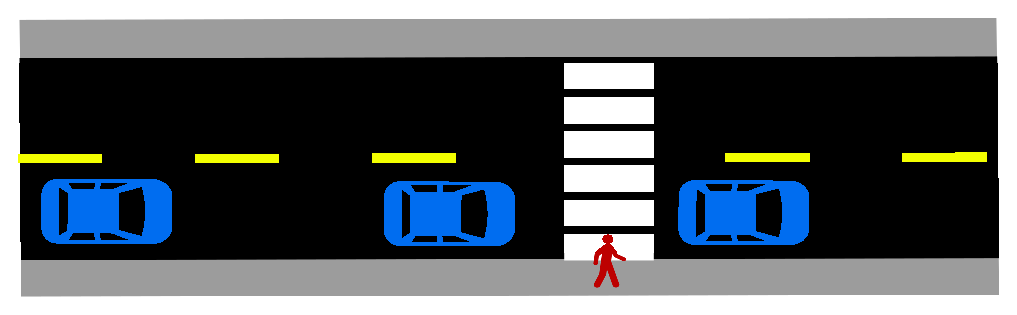
\includegraphics[width=3.5in]{figures/example.eps}
\caption{Schematic of pedestrian approaching a stream of traffic at a mid-block intersection.}
\label{fig:schematic}
\end{figure}

In general, right-of-way for uncontrolled intersections is complex. For example, nine states and the District of Columbia require motorists to stop when approaching a pedestrian in an uncontrolled crosswalk. Six states require a motorist to stop when a pedestrian is upon the same half of the roadway or within one lane of the lane that the motorist is traveling upon. Another nineteen states require a motorist to yield when a pedestrian is upon any portion of the roadway, and another 20 states mandate that motorists yield when a pedestrian is upon the same half of the roadway or approaching closely from the opposite side of the roadway \cite{NCSL}.

\subsection{Pedestrian Gap Acceptance}

One of the major factors that determines pedestrian crossing behavior is \textit{gap acceptance}, defined in this paper as:

\begin{align}
\mathrm{gap} = \frac{\mathrm{distance\hspace{1mm}to\hspace{1mm}crosswalk}}{\mathrm{vehicle\hspace{1mm}speed}}
\end{align} 

Also known as time to collision (TTC) - the safety gap is a measure of how much time there is before the vehicle would enter the crosswalk if it kept it's current speed constant. When faced with a stream of traffic at a crosswalk, a pedestrian inherently decides how much of a gap to accept before crossing. The average gap acceptance is reported in the literature to be between 3-7 seconds, meaning pedestrians usually do not cross if the vehicle would enter the crosswalk in under three seconds \cite{DiPietroCharlesMandKing1970}, and are very likely to cross when they have more than seven seconds \cite{Schmidt2009}. 

\subsection{Controller Objectives}

Given the multiple stakeholders present (the autonomous vehicle and its passengers, the pedestrian(s), and the other vehicles in the traffic stream), it is important to consider the values and needs of all participants when determining the objectives of a control framework. This paper determines controller objectives based on the three-part value sensitive design (VSD) framework proposed by Thornton et al. 
\cite{Thornton2018a} 







\section{Proposed Control Architecture}

\section{Evaluation Methodology and Simulation Results}

\section{Experimental Results}







\section{CONCLUSIONS}


\addtolength{\textheight}{-12cm}   % This command serves to balance the column lengths
                                  % on the last page of the document manually. It shortens
                                  % the textheight of the last page by a suitable amount.
                                  % This command does not take effect until the next page
                                  % so it should come on the page before the last. Make
                                  % sure that you do not shorten the textheight too much.

%%%%%%%%%%%%%%%%%%%%%%%%%%%%%%%%%%%%%%%%%%%%%%%%%%%%%%%%%%%%%%%%%%%%%%%%%%%%%%%%



%%%%%%%%%%%%%%%%%%%%%%%%%%%%%%%%%%%%%%%%%%%%%%%%%%%%%%%%%%%%%%%%%%%%%%%%%%%%%%%%



%%%%%%%%%%%%%%%%%%%%%%%%%%%%%%%%%%%%%%%%%%%%%%%%%%%%%%%%%%%%%%%%%%%%%%%%%%%%%%%%
\section*{APPENDIX}

Appendixes should appear before the acknowledgment.

\section*{ACKNOWLEDGMENT}





%%%%%%%%%%%%%%%%%%%%%%%%%%%%%%%%%%%%%%%%%%%%%%%%%%%%%%%%%%%%%%%%%%%%%%%%%%%%%%%%



\bibliographystyle{IEEEtran}
\bibliography{Bibliography}




\end{document}
